\chapter{Pacotes de Laboratório e o Uso de Metadados}
\label{cp:pacotes}

\section{Pacotes de Laboratório}
Dentro do âmbito da Engenharia de Software Experimental, a todo momento diversas pesquisas, técnicas e ferramentas são desenvolvidos para validar teses ou otimizar soluções, porém tais recursos ou informações isoladas não formam um corpo de
conhecimento consistente, faz-se necessário compartilhá-los entre os grupos de pesquisa por meio do uso de pacotes de laboratório.

Diversos pesquisadores relatam dificuldades na revisão de pacotes de laboratório, como problemas no compartilhamento de conhecimento entre grupos de pesquisa devido uma falta de padronização para a integração de um conhecimento novo e/ou isolado ao conhecimento comum \cite{Scatalon11}. Desta forma, é imprescindível uma boa definição e construção
de um pacote de laboratório com o uso de uma estrutura específica de simples compreensão, possibilitando inclusive o uso de ontologias para seu desenvolvimento.

\cite{Garcia08} propõem o uso de uma ontologia para a Engenharia de Software Experimental, que descreve os conceitos que compõem um pacote de laboratório para experimentos controlados, chamada \textit{ExperOntology}.
Uma ontologia é uma especificação formal explícita de uma conceitualização compartilhada, definindo parte de um domínio por meio de termos relevantes e seus respectivos relacionamentos, cuja estruturação é baseada por determinadas regras.

\begin{figure}[!htb]
\centering
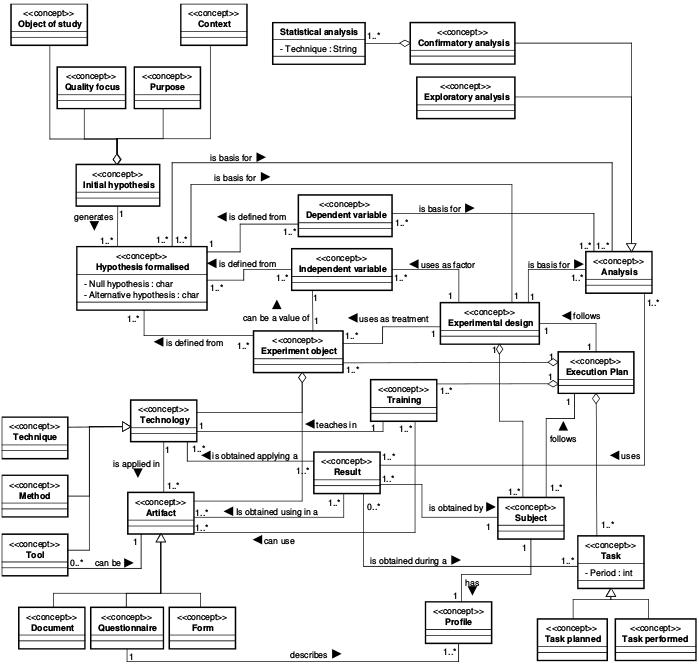
\includegraphics[scale=0.7]{images/onto.png}
\caption{Ontologia para Pacotes de Laboratório \cite{Garcia08}.}
\label{onto}
\end{figure}

A \textit{ExperOntology} visa à definir o principais conceitos de experimentos controlados desde a fase de definição até a análise de resultados, sendo importante ressaltar a evolução do experimento e o uso de pacotes de laboratório para armazenamento \cite{Garcia08}. 

Na Figura \ref{onto}, está descrito o processo de definição de um pacote de laboratório através da \textit{ExperOntology}. Inicialmente, é a elaborada de uma hipótese inicial, a qual juntamente com uma objeto de estudo e um contexto formam a formalização da hipótese. A partir deste ponto, são definidas as hipóteses nulas e alternativas, assim como as variáveis dependentes e independentes. Durante a fase de planejamento, são determinados os objetos de experimentação como as tecnologias e artefatos.

O principal objetivo das fases de definição e planejamento é estabelecer um modelo experimental que satisfaça todos os requisitos para a fase de análise. O resultado destas fases culmina em um modelo experimental e no plano de execução, o qual permite a definição de um ambiente controlado, realização de testes das hipóteses e minimização de impecílios para a validação do experimento.

\section{Bancos de Dados Não-Relacionais}
A partir da década 1960, diversas tecnologias para armazenamento de dados tem surgido, como o uso de documento de texto ou planilhas até sistema complexos de armazenamento de dados, como os \textit{SGBDs} (Sistemas Gerenciadores de Banco de Dados). 

Em meio a diversos modelos, como modelo rede e hierárquico, o modelo relacional tem sido utilizado em larga escala desde a sua criação em 1970. Este tem como característica a utilização de tabelas e tuplas para o armazenamento de dados assim como o uso de chaves primárias para garantia de identificação destes, dentro diversos outros recursos de restrição necessários, porém tornam a estruturação mais rígida \cite{brito2010bancos}.

Mediante ao crescente número de aplicações, o volume de dados tem aumentado exponencialmente nos últimos anos, o que tornou a mostra diversas limitações do modelo relacional principalmente quanto a eficiência na recuperação de dados e escalabilidade \cite{toth2011abordagem}.

Como alternativa, foram desenvolvidas novas soluções que priorizavam uma maior flexibilidade quanto ao armazenamento, desta forma, extinguindo certas regras presentes no modelo tradicional, o que fez surgir o Modelo Não-Relacional, o qual não tem como objetivo substituir o modelo relacional por completo, mas somente em casos em que seja mais vantajoso utilizá-lo, como em ambientes de Big Data. Alguns representantes de base não-relacionais são: Cassandra, Dynamo, MongoDB e BigTable.

Devido a inexistência de regras para a organização dos seus dados, diversas categorias de sistemas de banco de dados não-relacionais foram desenvolvidas, os principais serão detalhados abaixo:

\begin{itemize}
\item Orientados a Colunas (\textit{Column}): é a categoria que mais se aproxima do modelo relacional, porém todas as suas operações são voltadas para as colunas, ao invés das tuplas como no modelo relacional. O seu grande diferencial está na facilidade de inserção de novas colunas, ou seja, atributos com o sistema já em operação, conforme se tornarem necessários, sem apresentar problemas de esquema ou redundância de dados \cite{vaish2013getting}.

\item Armazenamento em Documentos (\textit{Document}): nesta categoria cada item é armazenado em um novo arquivo, em geral sua organização é feita através de estruturas chamadas coleções as quais são equivalentes as tabelas no modelo relacional, não possuem qualquer esquema, dois objetos de uma mesma coleção podem ter atributos diferentes, o que permite grande flexibilidade, sendo que cada registro é um arquivo. Os principais formatos de arquivos são JSON, XML, BSON e YAML \cite{vaish2013getting}.

\item Armazenamento Chave/Valor (\textit{Key/Value}): também muito semelhante a categoria anterior, porém seu armazenamento é feito com uso de uma chave, assemelhando-se a uma tabela Hash, ou um array associativo. Sua grande vantagem é busca por chaves, porém fornecer todas as demais operações comuns a base de dados \cite{vaish2013getting}.

\item Armazenamento em Grafos (\textit{Graph}): esta categoria tem foco nos relacionamentos entre as entidades, que no caso são os nós do grafo, permitindo o uso de múltiplas ligações entre os nós demonstrando características em comum, tal modelo pode ser ideal para redes sociais. Uma prática usual é mescla entre o banco de dados orientado a documentos e o orientado a grafos, tornando não obrigatória a presença de relacionamentos \cite{vaish2013getting}.

\end{itemize}

Abaixo segue uma tabela indicando alguns banco de dados não-relacionais e a respectiva tecnologia de armazenamento utilizada por estes:

\begin{table}[!htb]
\centering
\caption{Banco de Dados Não-Relacional e sua tecnologia de armazenamento.}
\begin{tabular}{c|c|c|c|c}
\hline
\textbf{Document} & \textbf{Key-Value} & \textbf{XML} & \textbf{Column} & \textbf{Graph}\\ 
\hline                               
MongoDB & Redis & BaseX & BigTable & Neo4J \\
\hline
CouchDB & Membase & eXist & Haddop/HBase & FlockDB \\
\hline
RavenDB & Voldemort & - & Cassandra & InfiniteGraph \\
\hline

\end{tabular}
\end{table}

Antes de se estabelecer uma comparação entre os modelos, é importante definir conceitos como que comporão esta análise:

\begin{itemize}
\item Escalonamento: este conceito, no contexto de banco de dados, consiste na capacidade em que uma base de dados tem de destruição tanto horizontal (\textit{scale out}), neste caso a estruturação do sistema é dividida em várias máquinas tanto por parte do banco de dados; quanto vertical (\textit{scale up}), no qual são realizadas melhorias de hardware em relação à processamento e armazenamento \cite{toth2011abordagem}.

\item Consistência: refere-se à capacidade de manter os dados de forma íntegra, de modo que evite quaisquer problemas no banco de dados possam modificar ou corromper os dados armazenados \cite{brito2010bancos}.

\item Disponibilidade: este quesito se refere a capacidade de acesso do usuário a referida informação, tanto em quesito de velocidade quanto de solicitação \cite{brito2010bancos}.

\end{itemize}

Por fim, de modo a esclarecer as reais vantagens e desvantagens do uso de uma base de dados não-relacional, a Tabela \ref{comparativo} demonstra um comparativo com o tradicional modelo relacional analisando os quesitos de consistência, escalonamento e disponibilidade \cite{brito2010bancos}.

\begin{table}[!t]
\label{comparativo}
\centering
\caption{Análise Comparativa do Modelo Relacional e Não-Relacional \cite{brito2010bancos}.}
\begin{tabular}{p{3.5cm}|p{5cm}|p{5cm}}
\hline
 & \textbf{Relacional} & \textbf{Não-Relacional} \\ 
\hline                               
\textbf{Escalonamento} & Possível, porém complexo devido à natureza estruturada do modelo, a adição de forma dinâmica e transparente de novos nós no modelo não é realizada de modo natural. & Uma das principais vantagens desse modelo, por não possuir nenhum tipo de esquema predefinido, o modelo possui maior flexibilidade o que favorece a inclusão transparente de outros elementos. \\
\hline
\textbf{Consistência} & Ponto mais forte do modelo relacional. As regras de consistência presentes propiciam uma maior grau de rigor quanto à consistência das informações. & Realizada de modo eventual no modelo: só garante que, se nenhuma atualização for realizada sobre o item de dados, todos os acessos a esse item devolverão o último valor atualizado. \\
\hline
\textbf{Disponibilidade} & Dada a dificuldade de se conseguir trabalhar de forma eficiente com a distribuição dos dados, esse modelo pode não suportar a demanda muito grande de informações do banco. & Outro fator fundamental do sucesso desse modelo. O alto grau de distribuição dos dados propicia que um maior número de solicitações aos dados seja atendida por parte do sistema e que o sistema fique menos tempo não-disponível. \\
\hline

\end{tabular}
\end{table}